% !TeX root = ../main.tex
\chapter{Background \& Related Work}
\label{chap:background}

This chapter gives an overview of the background software adopted while developing this work (\autoref{sec:background}), and shines light on the already existing similar work and adopted techniques on the subject (\autoref{sec:relatedwork}).


% ------------------------------------------------------------------------------
% Background
\section{Background}
\label{sec:background}

This section provides some background on the used software and the reason for its choice, what the Robot Operating System is (\autoref{ssec:ros}), and the simulation software adopted (\autoref{ssec:gazebo}). The research on runtime testing, the different techniques, and the difficulties of implementing it that already exist (\autoref{ssec:runtimetesting}), and also, the importance of invariant specification and its relation to Linear Temporal Logic (LTL) (\autoref{ssec:ltlinvariants}).


% ------------------------------------------------------------------------------
% ROS
\subsection{Robot Operating System}
\label{ssec:ros}

The Robot Operating System (ROS)~\cite{quigley2009ros} is an open-source framework with a vast collection of libraries, interfaces, and tools designed to help build robot software. ROS provides an abstraction between hardware and software. This abstraction helps developers easily connect the different robot components predominantly through messages sent through communication channels called \textit{topics} via a publish-subscribe architecture. A \textit{topic} decouples the production of information from its consumption, ROS nodes will subscribe and publish to relevant \textit{topics} and not know who they are comunicating with. Every \textit{topic} as a message type and can only receive messages of that type.

ROS has a modular architecture, is built with the purpose of cross-collaboration and easy development~\cite{ros-industrial}, is one hundred percent open source, available in multiple platforms, and ready for use across a wide array of robotics applications. For all these reasons, ROS is the norm for teaching robotics and is the basis for most robotics research, not only this but multiple companies rely on ROS for robotic development.

The ROS ecosystem ended up with a very strong \enquote{standard library} of packages that are used by almost everyone, and a large number of packages that don't belong to that standard library that are rarely used by anyone. This is generally seen as a bad thing in software ecosystems, but for this work, it is an advantage because it allows specifying the behavior of a smaller standard library and still be able to represent the behavior of a large number of ROS systems. Literature states that around eighty-two percent of ROS applications rely on packages released by a small subset of groups~\cite{9240632}.


% ------------------------------------------------------------------------------
% Gazebo
\subsection{Gazebo}
\label{ssec:gazebo}

Robotic systems simulation is an essential tool for testing robots' behavior. For this reason, Gazebo~\cite{koenig2004design} started with the idea of a high-fidelity simulator to simulate robots in any environment under mixed conditions.

Gazebo is an open-source 3D simulator that supports tools like sensors simulation, mesh management, and actuators control under different physics engines, among others, which makes it a simulator that very distinct robotic systems can use.

Gazebo was chosen as the simulator for the work to follow up the work done by Afsoon Afzal in GzScenic~\cite{AfzalGzScenic}, an automatic scene generation for the Gazebo simulator. In this way, it would be possible to have a tool to perform automatic tests in multiple arbitrarily generated scenarios.

\begin{figure}[htb]
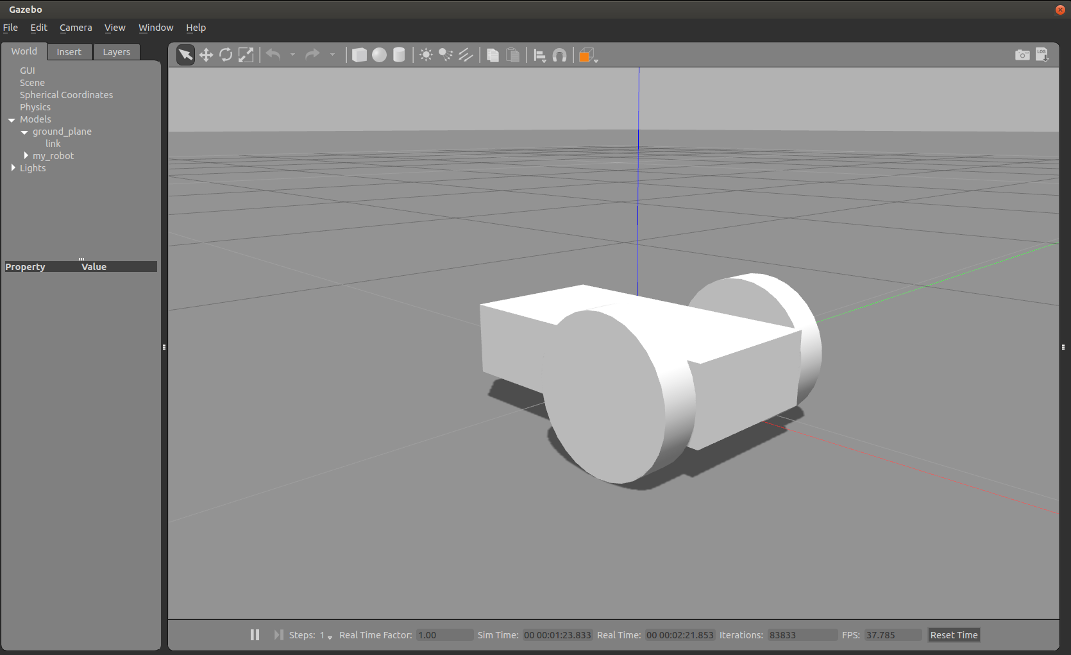
\includegraphics[width=\textwidth]{images/Gazebo_7_interface_mobile_base.png}
\caption{Gazebo 7's interface.} \label{fig:gazeboInterface}
\end{figure}

% ------------------------------------------------------------------------------
% Runtime Monitoring
\subsection{Runtime Testing}
\label{ssec:runtimetesting}

Runtime Testing is an analysis that takes place during the execution of a program, taking advantage of information from the running system to make inferences on if the observed information violates certain properties of the program.

Due to the mentioned unforeseen circumstances when executing robotic systems, runtime testing, although sometimes time-consuming, may be advantageous when identifying errors in these types of systems.

Implementing runtime monitoring adds load to the simulation since the computer has to allocate resources to the monitoring software. Therefore, not demanding excessive resources is essential when taking this approach.

Stadler, Vierhauser and Cleland-Huang \textit{"Towards flexible Runtime Monitoring Support for ROS-based Applications"}~\cite{stadler2022towards} pinpoint several challenges in developing runtime monitoring tools for robotic-based applications:

\begin{itemize}
    \item \textit{``Provisioning of an initial overview of the system structure.''}
    \item \textit{``Diversity and need to individually configure monitoring needs.''}
    \item \textit{``Only a subset of these properties likely need to be monitored on a continuous basis.''}
    \item \textit{``Data needs to be collected and analyzed differently.''}
    \item \textit{``Diverse types of constraints need to be defined and checked on the data.''}
    \item \textit{``Make the outcome of the runtime monitoring data and services accessible to the user.''}
\end{itemize}

These challenges are relevant in choosing which direction to take when specifying the DSL or implementing the monitoring tool for my approach. For instance, while I want the DSL to be intuitive and easily learned, it should also be capable of expressing all monitoring needs and giving an overview of the system. Also, identifying what type of data we need to monitor influences how the checking of the properties is computed.

%%Besides the method of monitoring chosen in this work, runtime testing can be implemented in other ways. For instance, Mithra~\cite{AfzalMithra} is a tool that provides an oracle for automated simulation-based testing relying on machine learning software, more specifically, a three-step multivariate time series clustering. \todo{Seems out of nowhere. I don't see the relationship to your work from this paragraph. What other methods are there?}


% ------------------------------------------------------------------------------
% Linear Temporal Logic and Invariants
\subsection{Linear Temporal Logic and Invariants}
\label{ssec:ltlinvariants}

An invariant represents a property that holds through the execution of the system. Having a set of invariants for a robotic system and asserting them at runtime makes it able to prove the correctness of the system.

Research on invariant checking~\cite{zizyte2021importance} demonstrates that important safety bugs in real-world autonomous robotic systems can be identified when representing safety violations of systems and monitoring them.

Linear temporal logic (LTL) is a branch of logic responsible for representing and reasoning about modalities in reference to time. 

As an approach for program verification, a formal system of temporal logic was suggested for both sequential and parallel programs~\cite{pnueli1977temporal}. LTL can be used as a method of model-checking~\cite{dwyer1998property} using its patterns as a form of property specification. It includes patterns such as "always", "finally", "until", "eventually", and others, which can be used to define invariants for program verification of robotics systems.


% ------------------------------------------------------------------------------
% Related Work
\section{Related Work}
\label{sec:relatedwork}

 Other monitoring frameworks that have already tried to implement similar runtime verification concepts are presented in \autoref{ssec:monitoringframeworks}.

% ------------------------------------------------------------------------------
% Monitoring Frameworks
\subsection{Monitoring Frameworks}
\label{ssec:monitoringframeworks}

Similar work on runtime monitoring that integrates with ROS already exists. 

ROSMonitoring~\cite{ferrando2020rosmonitoring} can monitor and log errors at the level of \textit{topic} (communication buses between the systems' components) malfunctioning, however, it was designed with portability and scalability in mind which means it is highly complex to use and can be not very user-friendly unless one is already knowledgeable of the subject.

ROSMonitoring also does not provide a ROS-oriented DSL, instead, it takes advantage of the already built and somewhat generic language Runtime Monitoring Language (RML)~\cite{rml} which doesn't provide the expressiveness and intuitiveness expected from a ROS-oriented invariant specification language. 

ROSRV~\cite{huang2014rosrv} is another tool that provides the runtime monitoring of ROS systems, however, ROSRV implements safety measures while the system is running, interfering with its normal execution. ROSRV lacks documentation on its functioning and usage. Additionally, ROSRV seems to have been discontinued since its last version is only capable of running under ROS Groovy Galapagos, which has not been supported since 2014.
